% This is part of Un soupçon de mathématique sans être agressif pour autant
% Copyright (c) 2014
%   Laurent Claessens
% See the file fdl-1.3.txt for copying conditions.

\documentclass{beamer}



\usepackage{latexsym}
\usepackage{amsfonts}
\usepackage{amsmath}
\usepackage{amsthm}
\usepackage{amssymb}
\usepackage{bbm}
\usepackage{mathrsfs}           
\usepackage{cases}

\usepackage[utf8]{inputenc}
\usepackage[T1]{fontenc}
\usepackage{multicol}

\usepackage{textcomp}
\usepackage{lmodern}
\usepackage[english,frenchb]{babel}


\usetheme{default}
\begin{document}

\begin{frame}{Théorème de Haga (Pythagore)}

    \begin{multicols}{2}

    \begin{center}        
        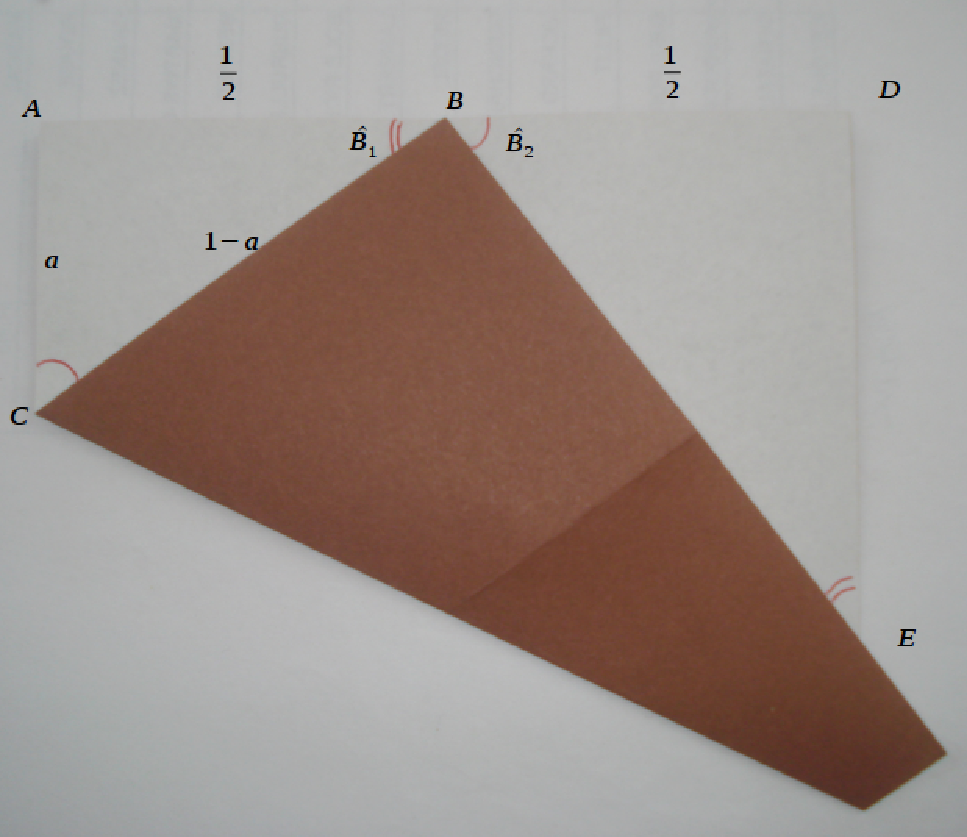
\includegraphics[width=5cm]{haga_coupe_anote}
    \end{center}


    Pythagore dans le triangle \( ABC\) : \( a^2+\left( \frac{ 1 }{2} \right)^2=(1-a)^2\).

    \( \Rightarrow \, a=\frac{ 3 }{ 8 }\).
    \end{multicols}

    
\end{frame}

\begin{frame}{Théorème de Haga (angles)}
    \begin{multicols}{2}

    \begin{center}        
        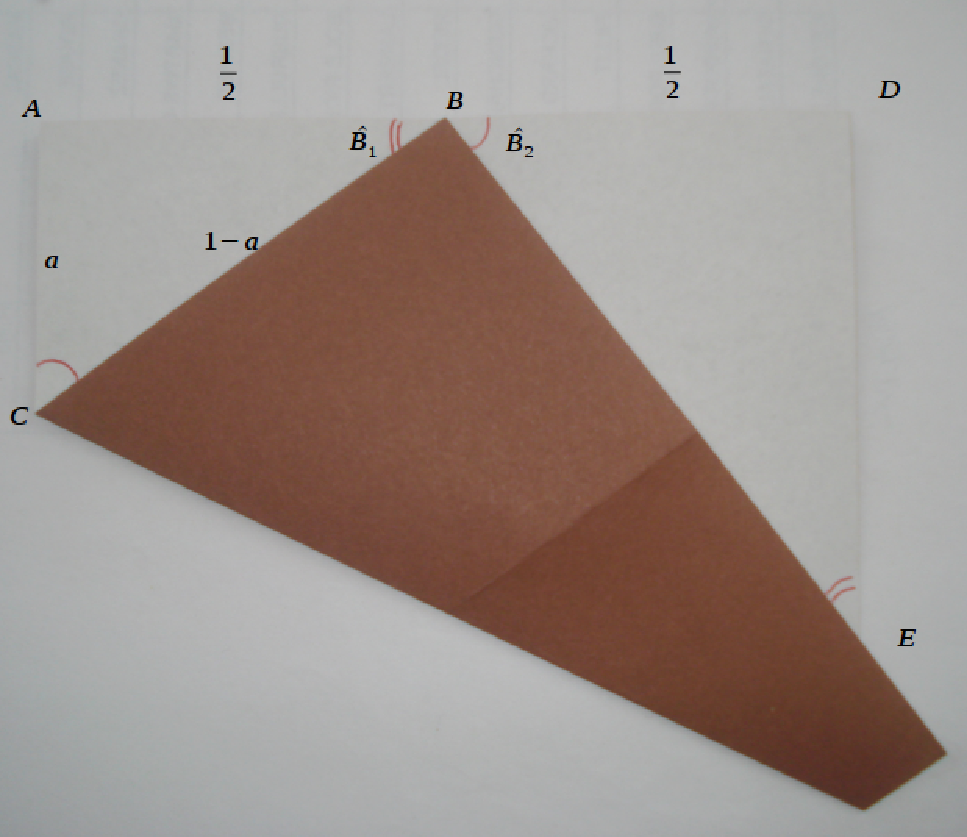
\includegraphics[width=5cm]{haga_coupe_anote}
    \end{center}

    \begin{subequations}
        \begin{numcases}{}
            \hat B_1+\hat B_2=90\\
            \hat B_1+\hat C=90\\
            \hat B_2+\hat E=90
        \end{numcases}
    \end{subequations}

    \( \Rightarrow \,   \hat B_2=\hat C \) et \( \hat B_1=\hat E\).
    \end{multicols}


    \begin{center}
        Les triangles \( ABC\) et \( BDE\) sont semblables.
    \end{center}
\end{frame}

\begin{frame}{Théorème de Haga (proportionalité)}
    \begin{multicols}{2}

    \begin{center}        
        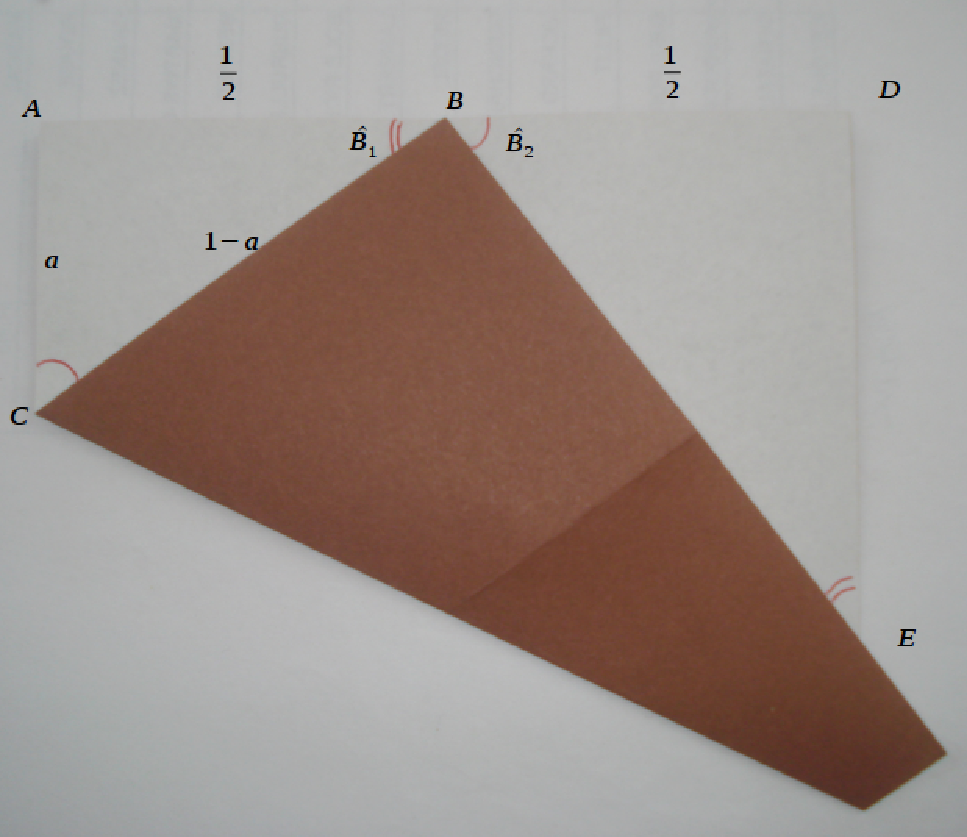
\includegraphics[width=5cm]{haga_coupe_anote}
    \end{center}

    \begin{equation}
        \frac{ DE }{ AB }=\frac{ BD }{ AC }
    \end{equation}
    \begin{equation}
        \frac{ DE }{ \frac{ 1 }{2} }=\frac{ \frac{ 1 }{2} }{ \frac{ 3 }{ 8 } }
    \end{equation}
    \begin{equation}
        2DE=\frac{ 4 }{ 3 }
    \end{equation}
    \begin{equation}
        DE=\frac{2}{ 3 }.
    \end{equation}
    \end{multicols}

\end{frame}

\end{document}
